\chapter{Background Theory}

\label{ch:background}

\section{Introduction}

We will cover how deep symbolic reinforcement learning extracts symbolic representations from raw input data, which will motivate a discussion of loss functions and the introduction of autoencoders. Seeing the limitations of the current approach in extracting symbolic representations, we can appreciate the recent development of $\beta$-VAE, a variant of the variational autoencoder used to learn disentangled representations. Finally, we can conclude by mentioning less technical matters, such as libraries and hardware used.

\section{Arithmetic in Neural Networks}

\subsection{Neurons}

\subsection{Activation Functions}

\subsection{Convolutions}

\subsection{Deconvolutions}

\subsection{Pooling and Up-Sampling}


\section{Loss functions}

The idea of image reconstruction plays a vital role throughout this project. Although it's possible to qualitatively compare the original to its reconstruction, it's important to be able to quantify the difference, which lends itself to automation. The loss function will quantify how similar two images are.

To compare loss functions, we'll use the MNIST data set. MNIST is a collection of $70,000$ black-and-white images of handwritten digits, with $60,000$ in the training set containing and $10,000$ in the test set. These images will be represented as vectors without loss of generality.

\subsection{Euclidean Distance}

The Euclidean distance between two vectors $\vec{x}$ and $\vec{y}$ is defined by $$\sqrt{\sum_{i}(x_i - y_i)^2}$$ where $x_i$ and $y_i$ are the $i^{th}$ components of $\vec{x}$ and $\vec{y}$ respectively.

Euclidean distance is an intuitive measure of the distance between two points in space. Unfortunately, this doesn't also translate to visual similarity, as illustrated by Doersch et al. \cite{Doersch2016}. Figure \ref{fig:eucledian_distance_a} is a digit drawn from the MNIST dataset, and Figures \ref{fig:eucledian_distance_b} and \ref{fig:eucledian_distance_c} are attempted reconstructions. Of the reconstructions, Figure \ref{fig:eucledian_distance_c} looks most like the original, but Figure \ref{fig:eucledian_distance_b} is closer in space.\\

\begin{figure}[!htb]
\centering
\minipage{0.32\textwidth}
\centering
  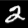
\includegraphics[width=0.8\linewidth]{background/eucledian_distance_a.png}
  \caption{}\label{fig:eucledian_distance_a}
\endminipage\hfill
\minipage{0.32\textwidth}
\centering
  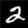
\includegraphics[width=0.8\linewidth]{background/eucledian_distance_c.png}
  \caption{}\label{fig:eucledian_distance_c}
\endminipage\hfill
\minipage{0.32\textwidth}%
\centering
  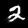
\includegraphics[width=0.8\linewidth]{background/eucledian_distance_b.png}
  \caption{}\label{fig:eucledian_distance_b}
\endminipage
\end{figure}

This leads to an alternative measure, binary cross-entropy, which gives a much better quantification of how visually similar two images are.

\subsection{Binary Cross-Entropy}
Consider a single black-and-white pixel with probability $p(0) = c$ of being $0$ and $p(1) = 1 - c$ of being $1$. Here $p(x)$ is a probability distribution over the possible pixel values $x \in \{0, 1\}$. Suppose a given model tries to learn the distribution described by $p(x)$, and says that the pixel has probability $q(0) = \hat{c}$ of being $0$ and $q(1) = 1 - \hat{c}$ of being $1$. The model is perfect if it learns the true distribution, that is, if $q(x) = p(x)$ for $x\in\{0,1\}$. We'd like to quantify how similar the distributions $p$ and $q$ are.

This is done by computing the binary cross-entropy between $p$ and $q$, which is defined by $$H(p,q) = -c\log\hat{c} - (1-c)\log(1-\hat{c})$$ To see how we may use this as a similarity measure among images, consider a $1\times1$ image. Normalising this image yields a pixel value in the interval $[0, 1]$, which may now be interpreted as a probability, corresponding to $c$ above. In the normalised reconstructed image, the pixel value corresponds to $\hat{c}$. We simply compute the binary cross-entropy to measure the similarity of these two distributions, and in turn, the similarity of the images themselves! (Note: we could have also assigned the probabilities to $1-y$ and $1-\hat{y}$ by symmetry of binary cross-entropy).

For images larger than $1 \times 1$, we may take the component-wise binary cross-entropy, then, for example, average the components. How the component-wise binary cross-entropies are combined to give a score single floating point number is the choice of the designer and will vary from problem to problem.

\section{Autoencoders}

An autoencoder is a neural network that learns a compression algorithm for its input data in an unsupervised manner \cite{Liou2008}. This is achieved by placing constraints on a hidden layer, called the latent space, and setting the target values to the input values, effectively learning the identity function. Since the network is trying to reconstruct the original input from the constrained latent space, over time the latent space corresponds to a meaningful compression of the network's input.

\begin{figure}[h!]
\centering
\captionsetup{justification=centering}
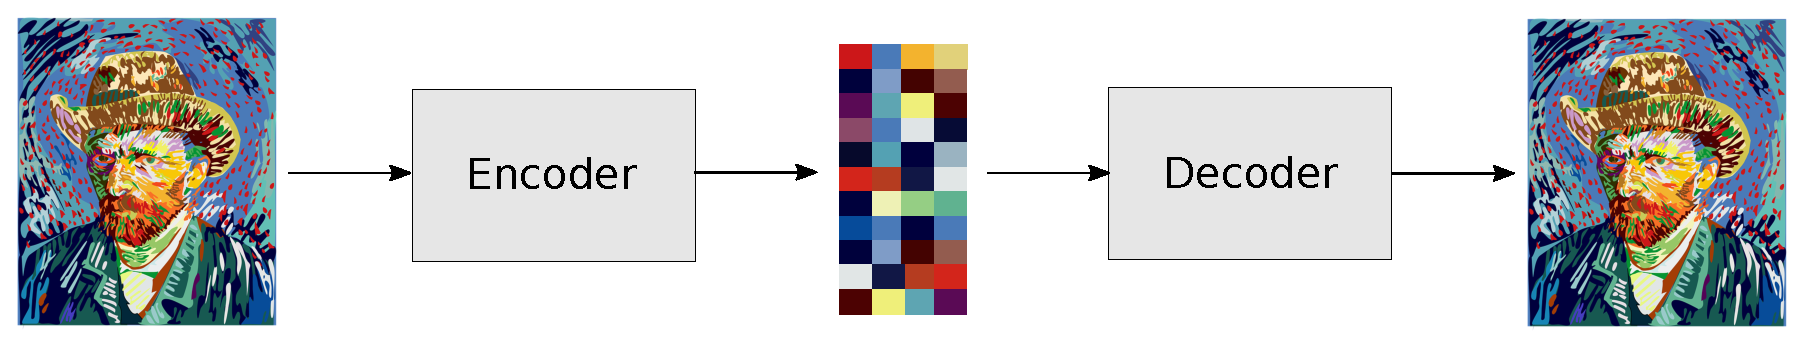
\includegraphics[scale=0.53]{background/autoencoder_black_box_architecture.eps}
\caption{A black-box description of an autoencoder. The autoencoder learns the identity function, and in turn, the encoder and decoder learn suitable encoding and decoding algorithms respectively.}
\label{fig:autoencoder_black_box_architecture}
\end{figure}

As before, we will use the MNIST data set to compare architectures. Unless specified in the example, the Adam optimiser is used with a learning rate of $1e-4$, the batch size is 1 and the loss function is binary cross-entropy. Intermediate layers use the ReLU activation function, while the final layer uses sigmoid.

\subsection{Fully-Connected Autoencoders}

In dense feed-forward neural networks we may place a constraint on the latent space by reducing the number of neurons, as shown in Figure \ref{fig:autoencoder_architecture}. Images must be flattened into vectors to be fed as input. Consequently, any spatial information is destroyed in dense feed-forward neural networks.

\begin{figure}[h!]
\centering
\captionsetup{justification=centering}
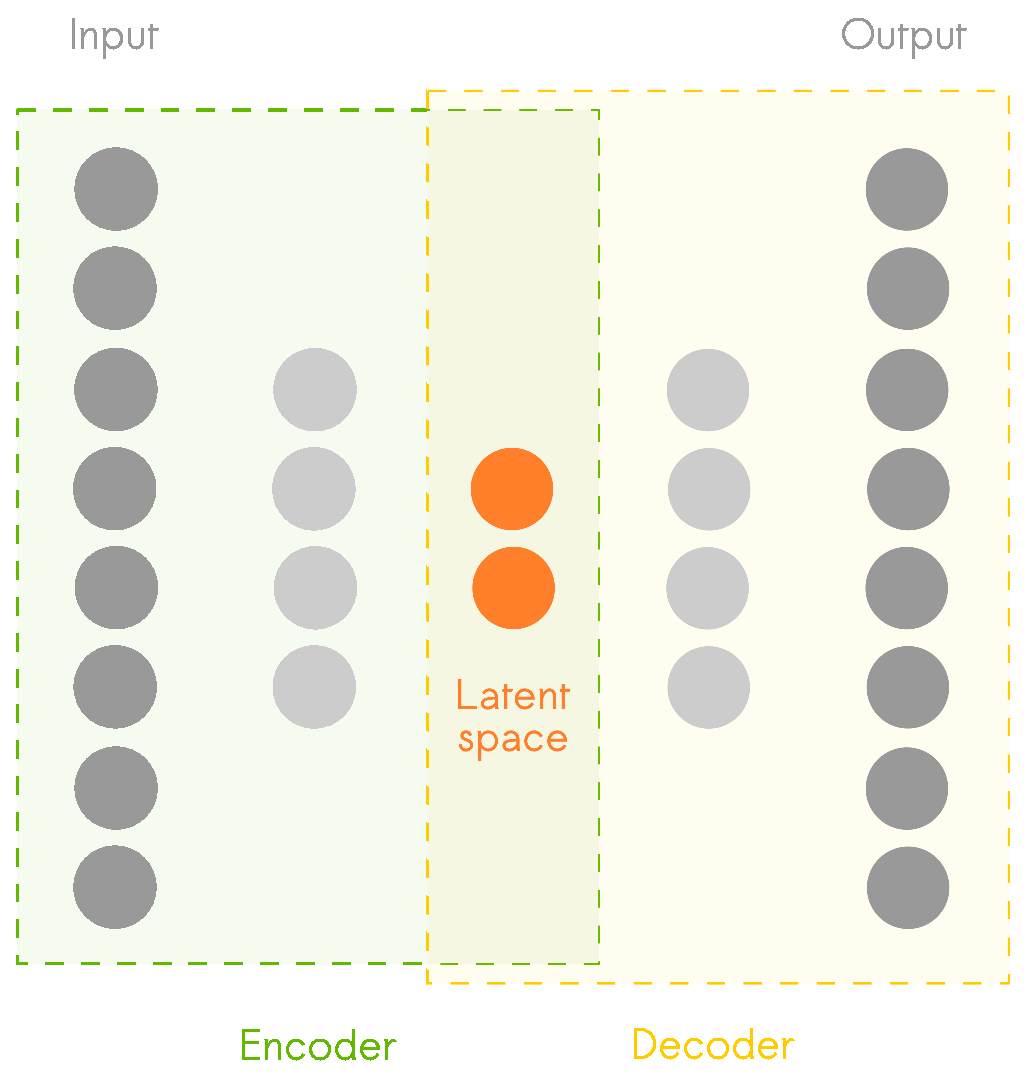
\includegraphics[scale=0.7]{background/autoencoder_architecture.eps}
\caption{An example architecture of a fully-connected autoencoder. The latent space is constrained by having fewer neurons than the input and output layers.}
\label{fig:autoencoder_architecture}
\end{figure}

An example architecture is given in Table \ref{tab:fully_connected_autoencoder_architecture}, which was trained on MNIST. Despite the latent space being $\sim4\%$ of the size of the input space, the network is capable of producing realistic reconstructions. For verification, a collection of samples from the dataset and their corresponding reconstructions are shown in Figure \ref{fig:fully_connected_autoencoder_mnist}.

\begin{table}[h!]
\centering
\captionsetup{justification=centering}
\begin{tabular}{@{}ll@{}}
\toprule
\textbf{Layer Type} & \textbf{Output Shape} \\ \midrule
InputLayer & (1, 28, 28) \\
Flatten & (784,) \\
Dense & (32,) \\
Dense & (784,) \\
Reshape & (1, 28, 28) \\ \bottomrule
\end{tabular}
\caption{A simple fully-connected autoencoder with one hidden layer. After 15 epochs, the validation score was recorded to be $71.94$.}
\label{tab:fully_connected_autoencoder_architecture}
\end{table}

\begin{figure}[h!]
\centering
\captionsetup{justification=centering}
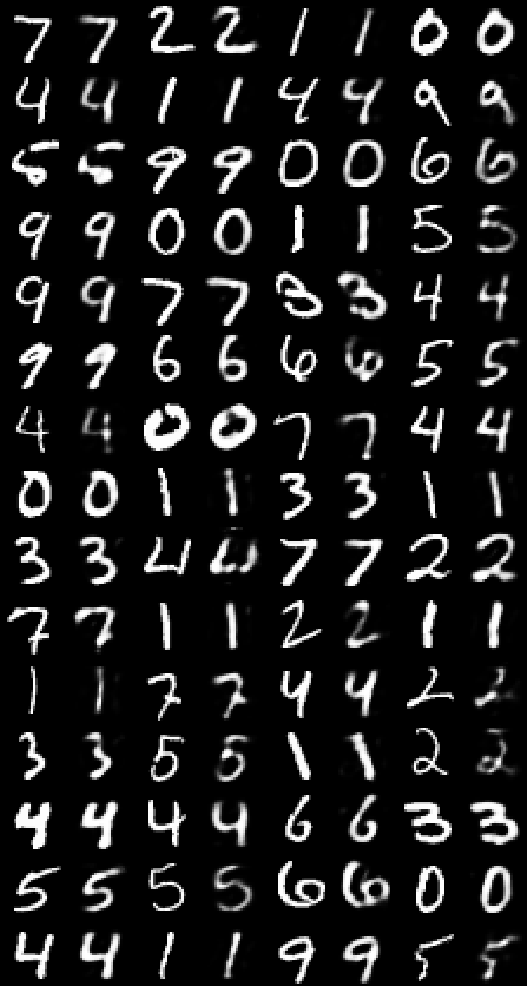
\includegraphics[scale=0.95]{background/fully_connected_autoencoder_mnist.png}
\caption{A collection of images from the MNIST data set and their respective reconstructions using the fully-connected autoencoder specified in Table \ref{tab:fully_connected_autoencoder_architecture}. The original MNIST images are in odd columns, and their reconstructions to their immediate right.}
\label{fig:fully_connected_autoencoder_mnist}
\end{figure}

\subsection{Fully-Convolutional Autoencoders}

In fully-convolutional feed-forward neural networks, we may place a constraint on the latent space by reducing the number and/or size of the filters, as shown in Figure \ref{fig:convolutional_autoencoder_architecture}. To compare the fully-convolutional autoencoder to the fully-connected, we'll train the architecture in Table \ref{tab:convolutional_autoencoder_architecture} on MNIST. As before, we'll compare the reconstructions to the originals, which can be found in Figure \ref{fig:convolutional_autoencoder_mnist}.

\begin{table}[h!]
\centering
\captionsetup{justification=centering}
\begin{tabular}{@{}ll@{}}
\toprule
\textbf{Layer Type} & \textbf{Output Shape} \\ \midrule
InputLayer & (1, 28, 28) \\
Conv2D & (32, 28, 28) \\
MaxPooling2D & (32, 14, 14) \\
Conv2D & (4, 14, 14) \\
MaxPooling2D & (4, 7, 7) \\
UpSampling2D & (4, 14, 14) \\
Conv2DTranspose & (32, 14, 14) \\
UpSampling2D & (32, 28, 28) \\
Conv2DTranspose & (1, 28, 28) \\ \bottomrule
\end{tabular}
\caption{A simple fully-convolutional autoencoder with 2D convolutions and max pooling, plus the corresponding deconvolutional layers. After 15 epochs, the validation score was recorded to be $64.89$.}
\label{tab:convolutional_autoencoder_architecture}
\end{table}

\begin{figure}[h!]
\centering
\captionsetup{justification=centering}
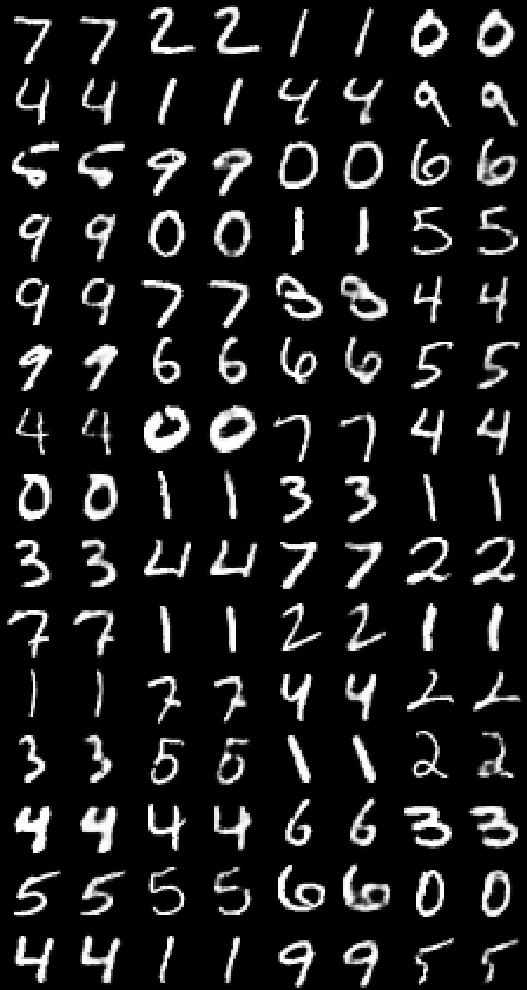
\includegraphics[scale=0.95]{background/fully_convolutional_autoencoder_mnist.png}
\caption{A collection of images from the MNIST data set and their respective reconstructions using the fully-convolutional autoencoder specified in Table \ref{tab:convolutional_autoencoder_architecture}. The original MNIST images are in odd columns, and their reconstructions to their immediate right.}
\label{fig:convolutional_autoencoder_mnist}
\end{figure}

\begin{figure}[h!]
\centering
\captionsetup{justification=centering}
\includegraphics[scale=0.6]{background/convolutional_autoencoder_architecture.eps}
\caption{An example architecture of a fully-convolutional autoencoder. The latent space is constrained by reducing the number and/or size of the filters.}
\label{fig:convolutional_autoencoder_architecture}
\end{figure}

Convolutional layers have been shown to be effective in tasks with images as input \cite{Krizhevsky2012, Zeiler2014, Szegedy2015}. This is because spatial information is preserved in convolutional layers, and the number of trainable parameters is far less in a convolutional layer than it is in a fully connected layer. Convolutional layers will be used from here on as we'll be using images as input.

\subsection{Variational Autoencoders}

The variational autoencoder is central to this project, and we'll therefore dedicate a considerable amount of time exploring it. First we'll relate the variational autoencoder to autoencoders seen earlier. This will lead us to formalise the proposed approach, after which we can develop a loss function and details its implementation.

\subsubsection{Introduction}
We've covered autoencoders that take an input $\vec{x}$ and output a reconstruction $\vec{\tilde{x}}$, after mapping the input to a lower-dimensional representation $\vec{z}$. Taking a probabilistic perspective gives an entirely new and exciting idea: each of the inputs $\vec{x}$ are actually samples from an unknown probability distribution $p(\vec{x})$ \cite{Doersch2016}. The variational autoencoder's aim is to learn $p(\vec{x})$ in an unsupervised manner, and consequently be able to generate new samples never seen in the original data set. The variational autoencoder is therefore suitably called a generative model.

\subsubsection{A Probabilistic Perspective}
Let $X = \{\vec{x}^{(i)}\}_{i=1}^{N}$ be the data set of $N$ independent and identically distributed samples of the variable $\vec{x}$. ($X$ may be a data set of images, for instance). Let us assume that these samples are generated by a random process with parameters $\vec{\theta^*}$ involving an unobserved latent variable $\vec{z}$ in the following way:\\

\begin{algorithm}
  \caption{Generate data set $X$}
  \begin{algorithmic}[1]
  \For{$i = 1 \to N$}
      \State $\vec{z}^{(i)} \sim p_{\vec{\theta}^*}(\vec{z})$ \quad\quad\quad\quad\quad\quad\quad\quad\quad\quad // Sample from true prior
      \State $\vec{x}^{(i)} \sim p_{\vec{\theta}^*}(\vec{x} | \vec{z}^{(i)})$ \quad\quad\quad\quad\quad\quad\quad\enspace\enspace\thinspace // Sample from true conditional
      \State Append $\vec{x}^{(i)}$ to $X$
  \EndFor
  \end{algorithmic}
  \label{alg:generate_data_set_x}
\end{algorithm}

We only observe the data set $X$ in this process. The parameters $\vec{\theta}^*$ and latent variables $Z = \{ \vec{z}^{(i)} \}_{i=1}^{N}$ are unknown to us. The variational autoencoder provides \cite{Kingma2014}:

\begin{enumerate}
\item ML or MAP estimation for the parameters $\vec{\theta}$.
\item An approximation of the latent variable $\vec{z}^{(i)}$ given $\vec{x}^{(i)}$ and set of parameters $\vec{\theta}$.
\item Approximate marginal inference of the variable $\vec{x}$.
\end{enumerate}


To be able to replicate this generative process, we have to estimate $\vec{\theta}^*$ without access to the latent values $Z$ \cite{Li2016}.

Let us assume that the prior $p_{\vec{\theta^*}}(\vec{z})$ and likelihood $p_{\vec{\theta^*}}(\vec{x}|\vec{z})$ are parameterised by the distributions $p_{\vec{\theta}}(\vec{z})$ and $p_{\vec{\theta}}(\vec{x}|\vec{z})$ respectively. Since we don't have access to the latent variables $Z$, we have to infer them. More precisely, we'd like to be able to calculate the posterior $p_{\vec{\theta}}(\vec{z}|\vec{x})$. By Bayes' theorem, the posterior is given by
\[
p_{\vec{\theta}}(\vec{z}|\vec{x}) = \frac{p_{\vec{\theta}}(\vec{x}|\vec{z})p_{\vec{\theta}}(\vec{z})}{p_{\vec{\theta}}(\vec{x})}
\]
However, due to the marginal likelihood
\[
p_{\vec{\theta}}(\vec{x}) = \int p_{\vec{\theta}}(\vec{z})p_{\vec{\theta}}(\vec{x}|\vec{z})d\vec{z}
\]
being intractable, we may not calculate $p_{\vec{\theta}}(\vec{z}|\vec{x})$ analytically \cite{Kingma2014}. Instead, we define an approximation $q_{\vec{\phi}}(\vec{z}|\vec{x})$ to the intractable posterior $p_{\vec{\theta}}(\vec{z}|\vec{x})$. We are now able to encode a given sample with $q_{\vec{\phi}}(\vec{z}|\vec{x})$, called the probabilistic encoder, and decode a given latent variable with $p_{\vec{\theta}}(\vec{x}|\vec{z})$, called the probabilistic decoder.

\subsubsection{Finding a Suitable Loss Function: the ELBO}
The probabilistic encoder $q_{\vec{\phi}}(\vec{z}|\vec{x})$ is used to approximate the intractable posterior $p_{\vec{\theta}}(\vec{z}|\vec{x})$. We'd like to be able to quantify how closley $q$ approximates $p$ so that we may write down a loss function. For this we use the KL divergence
\[
D_{KL}(q_{\vec{\phi}}(\vec{z}|\vec{x})||p_{\vec{\theta}}(\vec{z}|\vec{x})) = \mathbf{E}_{q_{\vec{\phi}}(\vec{z}|\vec{x})}\bigg[\log_{e}\frac{q_{\vec{\phi}}(\vec{z}|\vec{x})}{p_{\vec{\theta}}(\vec{z}|\vec{x})}\bigg]
\]
which measures how much information is lost when we represent $p$ with $q$ (measured in nats) \cite{Burnham2002}. Using the KL divergence, our problem now amounts to the optimisation problem \cite{Blei2016}:
\begin{align}
q_{\phi^*}(\vec{z}|\vec{x}) = \arg\min_{q_{\vec{\phi}}(\vec{z}|\vec{x})} D_{KL}(q_{\vec{\phi}}(\vec{z}|\vec{x})||p_{\vec{\theta}}(\vec{z}|\vec{x}))
\label{eq:kl_divergence_optimisation_problem}
\end{align}
To see how we can start to minimise the KL divergence, we'll start by rewriting it in a different form:
\begin{align}
D_{KL}(q_{\vec{\phi}}(\vec{z}|\vec{x})||p_{\vec{\theta}}(\vec{z}|\vec{x})) &= \mathbf{E}_{q_{\vec{\phi}}(\vec{z}|\vec{x})}\bigg[\log_{e}\frac{q_{\vec{\phi}}(\vec{z}|\vec{x})}{p_{\vec{\theta}}(\vec{z}|\vec{x})}\bigg] \nonumber\\
&= \mathbf{E}_{q_{\vec{\phi}}(\vec{z}|\vec{x})}\big[\log_{e}q_{\vec{\phi}}(\vec{z}|\vec{x})\big] - \mathbf{E}_{q_{\vec{\phi}}(\vec{z}|\vec{x})}\big[{\log_ep_{\vec{\theta}}(\vec{z}|\vec{x})}\big] \nonumber\\
&= \mathbf{E}_{q_{\vec{\phi}}(\vec{z}|\vec{x})}\big[\log_{e}q_{\vec{\phi}}(\vec{z}|\vec{x})\big] - \mathbf{E}_{q_{\vec{\phi}}(\vec{z}|\vec{x})}\big[{\log_ep_{\vec{\theta}}(\vec{z},\vec{x})}\big] + \mathbf{E}_{q_{\vec{\phi}}(\vec{z}|\vec{x})}\big[\log_ep_{\vec{\theta}}(\vec{x})\big] \nonumber\\
&= \mathbf{E}_{q_{\vec{\phi}}(\vec{z}|\vec{x})}\bigg[\log_{e}\frac{q_{\vec{\phi}}(\vec{z}|\vec{x})}{{p_{\vec{\theta}}(\vec{z},\vec{x})}}\bigg] + \log_ep_{\vec{\theta}}(\vec{x})
\label{eq:kl_divergence}
\end{align}
Here we see that the KL divergence depends on the intractable marginal likelihood $p_{\vec{\theta}}(\vec{x})$! There's no way we can minimise it if we can't write down $p_{\vec{\theta}}(\vec{x})$. However, we can get around this: we'll minimise the KL divergence, but not directly. Instead, we try to find a quantity which we can maximise, and show that in turn this minimises the KL divergence. The trick is not obvious, but is simply done by finding a lower bound on the log marginal likelihood.

Using Jensen's inequality
\[
f(\mathbf{E}\big[X\big]) \geq \mathbf{E}\big[ f(X) \big]
\]
we can write down a lower bound on the log marginal likelihood:
\begin{align}
\log_ep_{\vec{\theta}}(\vec{x}) &= \log_e\int p_{\vec{\vec{\theta}}}(\vec{x}, \vec{z})d\vec{z} \nonumber\\
&= \log_e\int p_{\vec{\theta}}(\vec{x}, \vec{z}) \frac{q_{\vec{\phi}}(\vec{z}|\vec{x})}{q_{\vec{\phi}}(\vec{z}|\vec{x})} d\vec{z} \nonumber\\
&= \log_e\mathbf{E}_{q_{\vec{\phi}}(\vec{z}|\vec{x})}\bigg[  \frac{p_{\vec{\theta}}(\vec{x}, \vec{z})}{q_{\vec{\phi}}(\vec{z}|\vec{x})} \bigg]\nonumber\\
&\geq \mathbf{E}_{q_{\vec{\phi}}(\vec{z}|\vec{x})}\bigg[  \log_e\frac{p_{\vec{\theta}}(\vec{x}, \vec{z})}{q_{\vec{\phi}}(\vec{z}|\vec{x})} \bigg] \nonumber\\
&:= \mathcal{L}(\vec{\theta}, \vec{\phi}; \vec{x})
\label{eq:elbo}
\end{align}
Expression (\ref{eq:elbo}) is called the $ELBO$ (short for expected lower bound) \cite{Blei2011, Kingma2014}.

How does the $ELBO$ help us with minimising the KL divergence? First recall the alternative form of the KL divergence written in Equation (\ref{eq:kl_divergence}):
\[
D_{KL}(q_{\vec{\phi}}(\vec{z}|\vec{x})||p_{\vec{\theta}}(\vec{z}|\vec{x})) = \mathbf{E}_{q_{\vec{\phi}}(\vec{z}|\vec{x})}\bigg[\log_{e}\frac{q_{\vec{\phi}}(\vec{z}|\vec{x})}{{p_{\vec{\theta}}(\vec{z},\vec{x})}}\bigg] + \log_ep_{\vec{\theta}}(\vec{x})
\]
Writing this in terms of the $ELBO$ we have:
\[
D_{KL}(q_{\vec{\phi}}(\vec{z}|\vec{x})||p_{\vec{\theta}}(\vec{z}|\vec{x})) = -\mathcal{L}(\vec{\theta}, \vec{\phi}; \vec{x}) + \log_ep_{\vec{\theta}}(\vec{x})
\]
Since the KL divergence is the negative of the $ELBO$ up to an additive constant (with respect to $q$), minimising the KL divergence is equivalent to maximising the $ELBO$ \cite{Blei2016}.

\subsubsection{Maximising the ELBO in a Neural Network}
We've found that we can maximise the $ELBO$ to minimise the KL divergence between the approximation $q_{\vec{\phi}}(\vec{z}|\vec{x})$ and the intractable posterior $p_{\vec{\theta}}(\vec{z}|\vec{x})$. The $ELBO$ may be written as follows:
\begin{align}
\mathcal{L}(\vec{\theta}, \vec{\phi}; \vec{x}) &= \mathbf{E}_{q_{\vec{\phi}}(\vec{z}|\vec{x})}\bigg[  \log_e\frac{p_{\vec{\theta}}(\vec{x}, \vec{z})}{q_{\vec{\phi}}(\vec{z}|\vec{x})} \bigg] \\
&= -\mathbf{E}_{q_{\vec{\phi}}(\vec{z}|\vec{x})}\bigg[ \log_e\frac{q_{\vec{\phi}}(\vec{z}|\vec{x})}{p_{\vec{\theta}}(\vec{x}, \vec{z})} \bigg] \\
&= -\mathbf{E}_{q_{\vec{\phi}}(\vec{z}|\vec{x})}\bigg[ \log_e\frac{q_{\vec{\phi}}(\vec{z}|\vec{x})}{p_{\vec{\theta}}(\vec{x} | \vec{z}) p_{\vec{\theta}}(\vec{z})} \bigg] \\
&= -\mathbf{E}_{q_{\vec{\phi}}(\vec{z}|\vec{x})}\bigg[ \log_e\frac{q_{\vec{\phi}}(\vec{z}|\vec{x})}{p_{\vec{\theta}}(\vec{z})} \bigg] +  \mathbf{E}_{q_{\vec{\phi}}(\vec{z}|\vec{x})}\big[\log_e p_{\vec{\theta}}(\vec{x} | \vec{z}) \big]\\
&= -D_{KL}(q_{\vec{\phi}}(\vec{z}|\vec{x}) || p_{\vec{\theta}}(\vec{z})) + \mathbf{E}_{q_{\vec{\phi}}(\vec{z}|\vec{x})}\big[\log p_{\vec{\theta}}(\vec{x} | \vec{z}) \big]
\label{eq:elbo_reconstruction_kl_divergence}
\end{align}
Thus for a single data point $\vec{x}^{(i)}$, the $ELBO$ becomes
\begin{equation}
\mathcal{L}(\vec{\theta}, \vec{\phi}; \vec{x}^{(i)}) = -D_{KL}(q_{\vec{\phi}}(\vec{z}|\vec{x}^{(i)}) || p_{\vec{\theta}}(\vec{z})) + \mathbf{E}_{q_{\vec{\phi}}(\vec{z}|\vec{x}^{(i)})}\big[\log p_{\vec{\theta}}(\vec{x}^{(i)} | \vec{z}) \big]
\end{equation}
In this form, the $ELBO$ is 

\begin{figure}[h!]
\centering
\captionsetup{justification=centering}
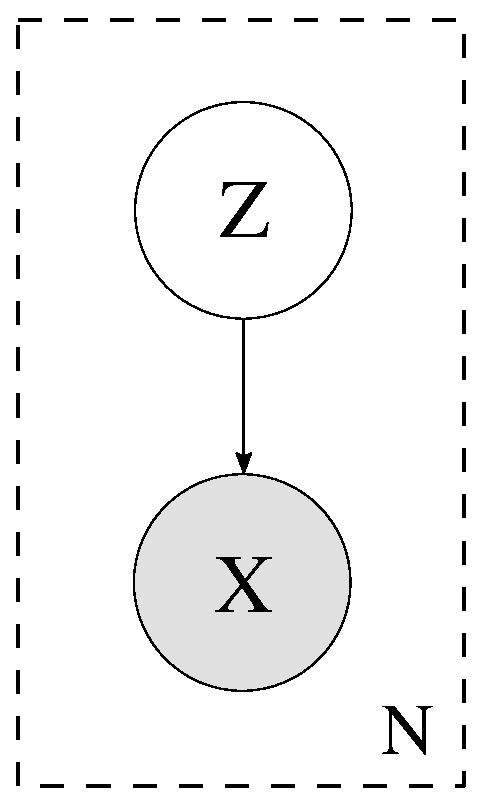
\includegraphics[scale=0.45]{background/variational_autoencoders_plate_model.eps}
\caption{An example architecture of a fully-convolutional autoencoder. The latent space is constrained by reducing the number and/or size of the filters.}
\label{fig:variational_autoencoder_plate_model}
\end{figure}
